
\documentclass[compress,aspectratio=1610]{beamer}

\usepackage[english]{babel}
\usepackage[english]{isodate}
\isodate
\usepackage{multicol}
\usepackage[italic]{hepnicenames}
\usepackage{progressbar}
\usepackage{siunitx}
\usepackage{booktabs}
\usepackage{appendixnumberbeamer}

\usetheme{vertex}

\linespread{1.1}

\usepackage{tikz}
\usetikzlibrary{arrows,shapes}
\usetikzlibrary{trees}
\usetikzlibrary{matrix,arrows} 				% For commutative diagram
\usetikzlibrary{positioning}				% For "above of=" commands
\usetikzlibrary{calc,through}				% For coordinates
\usetikzlibrary{decorations.pathreplacing}  % For curly braces
\usetikzlibrary{shapes.misc}
\tikzset{cross/.style={cross out, draw=red, fill=none, line width=1pt, minimum size=2*(#1-\pgflinewidth), inner sep=0pt, outer sep=0pt}, cross/.default={4pt}}
\usepackage{pgffor}							% For repeating patterns

\usetikzlibrary{decorations.pathmorphing}	% For Feynman Diagrams
\usetikzlibrary{decorations.markings}
\tikzset{%
	% >=stealth', %%  Uncomment for more conventional arrows
  vector/.style={decorate, decoration={snake}, draw},
	provector/.style={decorate, decoration={snake,amplitude=2.5pt}, draw},
	antivector/.style={decorate, decoration={snake,amplitude=-2.5pt}, draw},
  fermion/.style={draw=black, postaction={decorate},
      decoration={markings,mark=at position .55 with {\arrow[draw=black]{>}}}},
  fermionbar/.style={draw=black, postaction={decorate},
      decoration={markings,mark=at position .55 with {\arrow[draw=black]{<}}}},
  fermionnoarrow/.style={draw=black}
}

\title{A first look at \HepProcess{\PB\to\APD\Pmu\Pmu}}
\subtitle{Theory, Data and Selection}
\date{\today}
\author{Igor Babuschkin}

\begin{document}

\maketitle

\begin{frame}{Introduction}
  \textbf{Progress:}

  \begin{center}
  October 2014\raisebox{-.3\height}{\hspace{1em}\progressbar[subdivisions=12,width=6cm,heightr=2]{0.15}}\hspace{1em}September 2015
  \end{center}
  
  \textbf{Topics:}
  \begin{itemize}
    \item Theory (Diagram, Predictions)
    \item Dataset (Stripping, Blinding)
    \item Selection (Preselection, Classification)
  \end{itemize}
\end{frame}

\begin{frame}{Theory}
  \begin{minipage}{0.75\textwidth}
  \begin{itemize}
    \item Paper by \textit{Evans et al.} (2000)
    \item OPE and Heavy Quark Expansion
    \item Result depends on matrix elements $β$ and $β_8$
    \item A few crude assumptions made (in absence of Lattice QCD)
    \item Prediction:
      \begin{align*}
        \mathrm{Br}(\HepProcess{\APBzero \to \PDz e^+ e^-})|_{q^2 > \SI{1}{GeV}} &= \num{2.6e-9} \\
        \mathrm{Br}(\HepProcess{\APBzero \to \PDstar e^+ e^-})|_{q^2 > \SI{1}{GeV}} &= \num{1.4e-8}
      \end{align*}
    \item Might be enhanced if assumptions unjustified
    \item Idea: Also look at \PDstar
  \end{itemize}
  \end{minipage}
  \begin{minipage}{0.15\textwidth}
  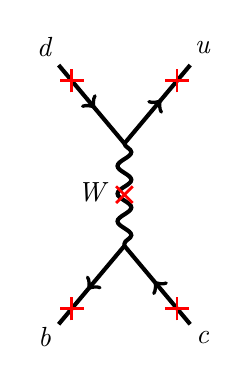
\begin{tikzpicture}[
    line width=1.5 pt,
    scale=1.3,
    decoration={
      markings,
      mark=at position 0.2 with {\node[cross,rotate=45] {};}}
    ] 
    \begin{scope}[rotate=90]
      \draw[fermion] (-140:1)--(0,0);
        \draw[fermionbar] (140:1)--(0,0);
        \draw[vector] (0:1)--(0,0);
        \node[cross] at (0:0.5) {};
        \node at (-140:1.2) {\Pqc};
        \node at (140:1.2) {\Pqb};
        \node at (.5,.3) {\PW};	
      \begin{scope}[shift={(1,0)}]
        \draw[fermionbar] (-40:1)--(0,0);
        \draw[fermion] (40:1)--(0,0);
        \node at (-40:1.2) {\Pqu};
        \node at (40:1.2) {\Pqd};	
      \end{scope}
    \end{scope}
  \end{tikzpicture}
  \end{minipage}
\end{frame}

\begin{frame}{Dataset: Stripping}
  \begin{minipage}{0.45\textwidth}
  \begin{itemize}
    \item Stripping line: \texttt{Dimuon/B2XMuMu\_Line}
    \item Data from 2011 and 2012 (\SI{3}{\per\femto\barn})
    \item Slightly over \num{e6} events
  \end{itemize}
  \end{minipage}
  \begin{minipage}{0.54\textwidth}
  \centering
  {\footnotesize
  \begin{tabular}{l l}
    \toprule
    Candidate & Selection \\
    \midrule
    \PB & $\text{IP}\:\chi^2 < 16 \text{(best PV)}$ \\
        & $\SI{4600}{MeV/c^2} < M < \SI{7000}{MeV/c^2}$ \\
        & $\text{DIRA angle} < \SI{14}{mrad}$ \\
        & $\text{flight distance}\:\chi^2 > 121$ \\
        & $\text{vertex}\:\chi^2 / \text{ndf} < 8$ \\
    \Pmuon\APmuon & $m(\Pmuon\APmuon) < \SI{7100}{MeV/c^2}$ \\
        & $\text{vertex}\:\chi^2/\text{ndf} < 9$ \\
        & \texttt{isMuon} \\
        & $\text{DLL}_{\Pmu\Ppi} > -3$ \\
    \PDzero & $\text{ADAMASS}(\PDzero) < \SI{100}{MeV/c^2}$ \\
            & $\text{vertex}\:\chi^2 < 10$ \\
    \text{tracks} & $\text{ghost prob} < \num{0.4}$ \\
                  & $\text{min IP}\:\chi^2 > 9$ \\
    GEC & $\text{SPD Mult.} < 600$ \\
    \bottomrule
  \end{tabular}}
  \end{minipage}
  
  % Table with stripping cuts
\end{frame}

\begin{frame}{Dataset: Blinding}
  \centering
  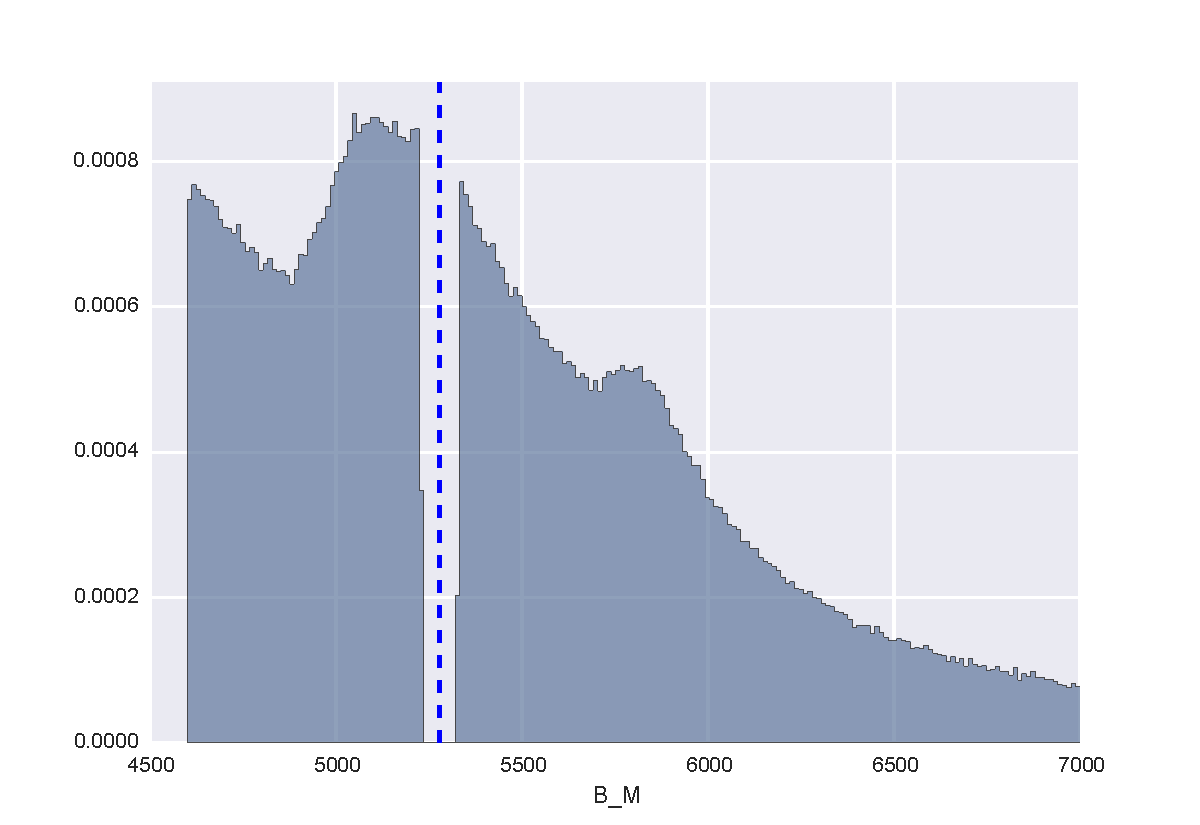
\includegraphics[page=1,width=0.8\textwidth]{figures/blinded.pdf}
\end{frame}

\begin{frame}{Dataset: Trigger lines}
  \centering
  \begin{tabular}{l}
    \toprule
    Trigger lines \\
    \midrule
    \texttt{B\_L0MuonDecision} \\
    \texttt{B\_Hlt1TrackAllL0Decision} \\
    \texttt{B\_Hlt1TrackMuonDecision} \\
    \texttt{B\_Hlt2Topo\{2,3,4\}BodyBBDTDecision} \\
    \texttt{B\_Hlt2TopoMu\{2,3,4\}BodyBBDTDecision} \\
    \texttt{B\_Hlt2SingleMuonDecision} \\
    \texttt{B\_Hlt2DiMuonDetachedDecision} \\
    \bottomrule
  \end{tabular}
\end{frame}

\begin{frame}{Dataset}
  \centering
  \makebox[\textwidth][c]{%
  \includegraphics[page=2,width=0.56\textwidth]{figures/blinded.pdf}%
  \includegraphics[page=3,width=0.56\textwidth]{figures/blinded.pdf}%
  }
\end{frame}

\begin{frame}{Selection: \PJpsi cuts}
  \centering
  \makebox[\textwidth][c]{%
  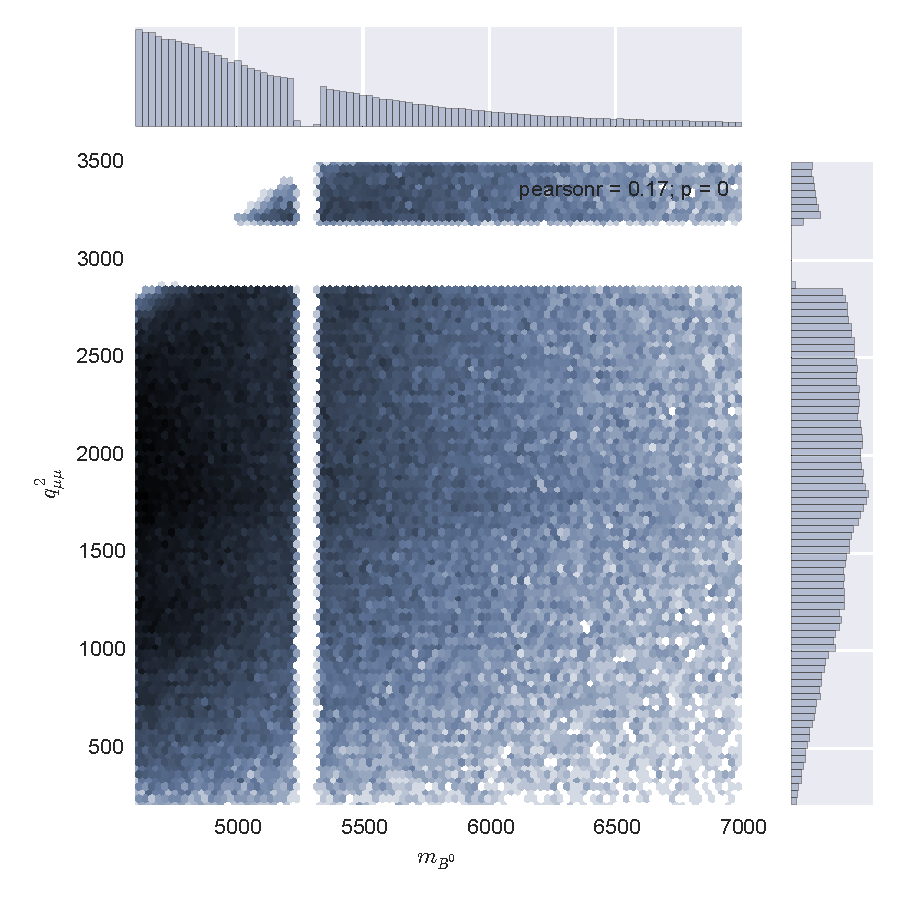
\includegraphics[page=1,width=0.56\textwidth]{figures/select.pdf}%
  \includegraphics[page=2,width=0.56\textwidth]{figures/select.pdf}%
  }
\end{frame}

\begin{frame}{Selection: PID cuts}
  \centering
  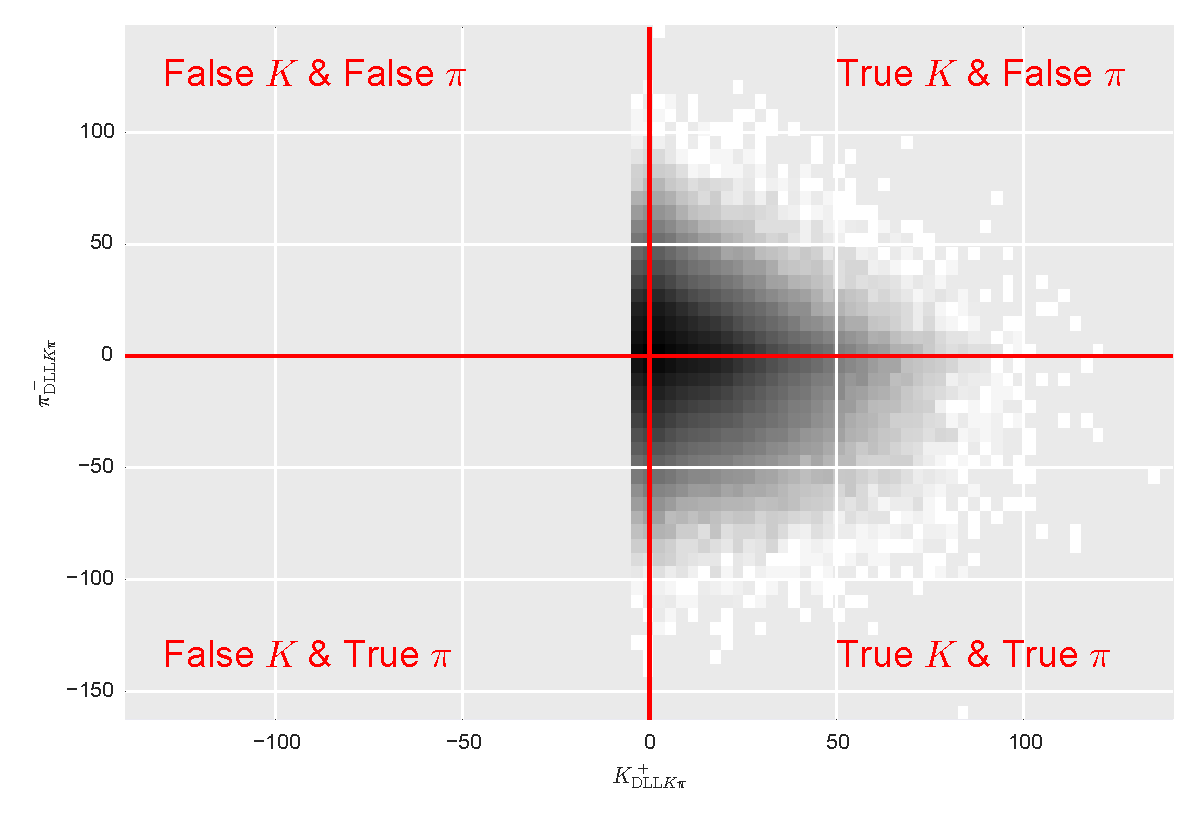
\includegraphics[width=0.8\textwidth]{figures/pid_plot.pdf}
\end{frame}

\begin{frame}{Selection: Classifier}
  \begin{minipage}{0.6\textwidth}
    \begin{itemize}
      \item Classifier: AdaBoost
      \item Trained on
        \begin{itemize}
          \item upper \PBz mass sideband (background)
          \item \HepProcess{\PBzero\to\APDzero\Pmu\Pmu} PHSP Monte Carlo (signal)
        \end{itemize}
      \item Feature set can still be improved (see rhs)
    \end{itemize}
  \end{minipage}
  \begin{minipage}{0.38\textwidth}
  \centering
  {\footnotesize
  \begin{tabular}{l}
  \toprule
  Variables \\
  \midrule
  \texttt{B\_TAU} \\
  \texttt{B\_ISOLATION\_BDT\_Soft} \\
  \texttt{B\_ENDVERTEX\_CHI2} \\
  \texttt{B\_DIRA\_OWNPV} \\
  \texttt{D\textasciitilde0\_DIRA\_OWNPV} \\
  \texttt{Kplus\_ProbNNpi} \\
  \texttt{Kplus\_ProbNNk} \\
  \texttt{Kplus\_ProbNNp} \\
  \texttt{piminus\_ProbNNk} \\
  \texttt{piminus\_ProbNNp} \\
  \texttt{piminus\_ProbNNpi} \\
  \texttt{muplus\_ProbNNmu} \\
  \texttt{muminus\_ProbNNmu} \\
  \texttt{*\_TRACK\_GhostProb} \\
  \bottomrule
  \end{tabular}}
  \end{minipage}
\end{frame}

\begin{frame}{Classifier: Feature correlation matrix}
  \begin{minipage}{0.29\textwidth}
    \begin{itemize}
      \item Data mostly unprepared
      \item No transformations applied (log/acos)
      \item Error values left in (idea: impute)
    \end{itemize}
  \end{minipage}
  \begin{minipage}{0.7\textwidth}
    \centering
    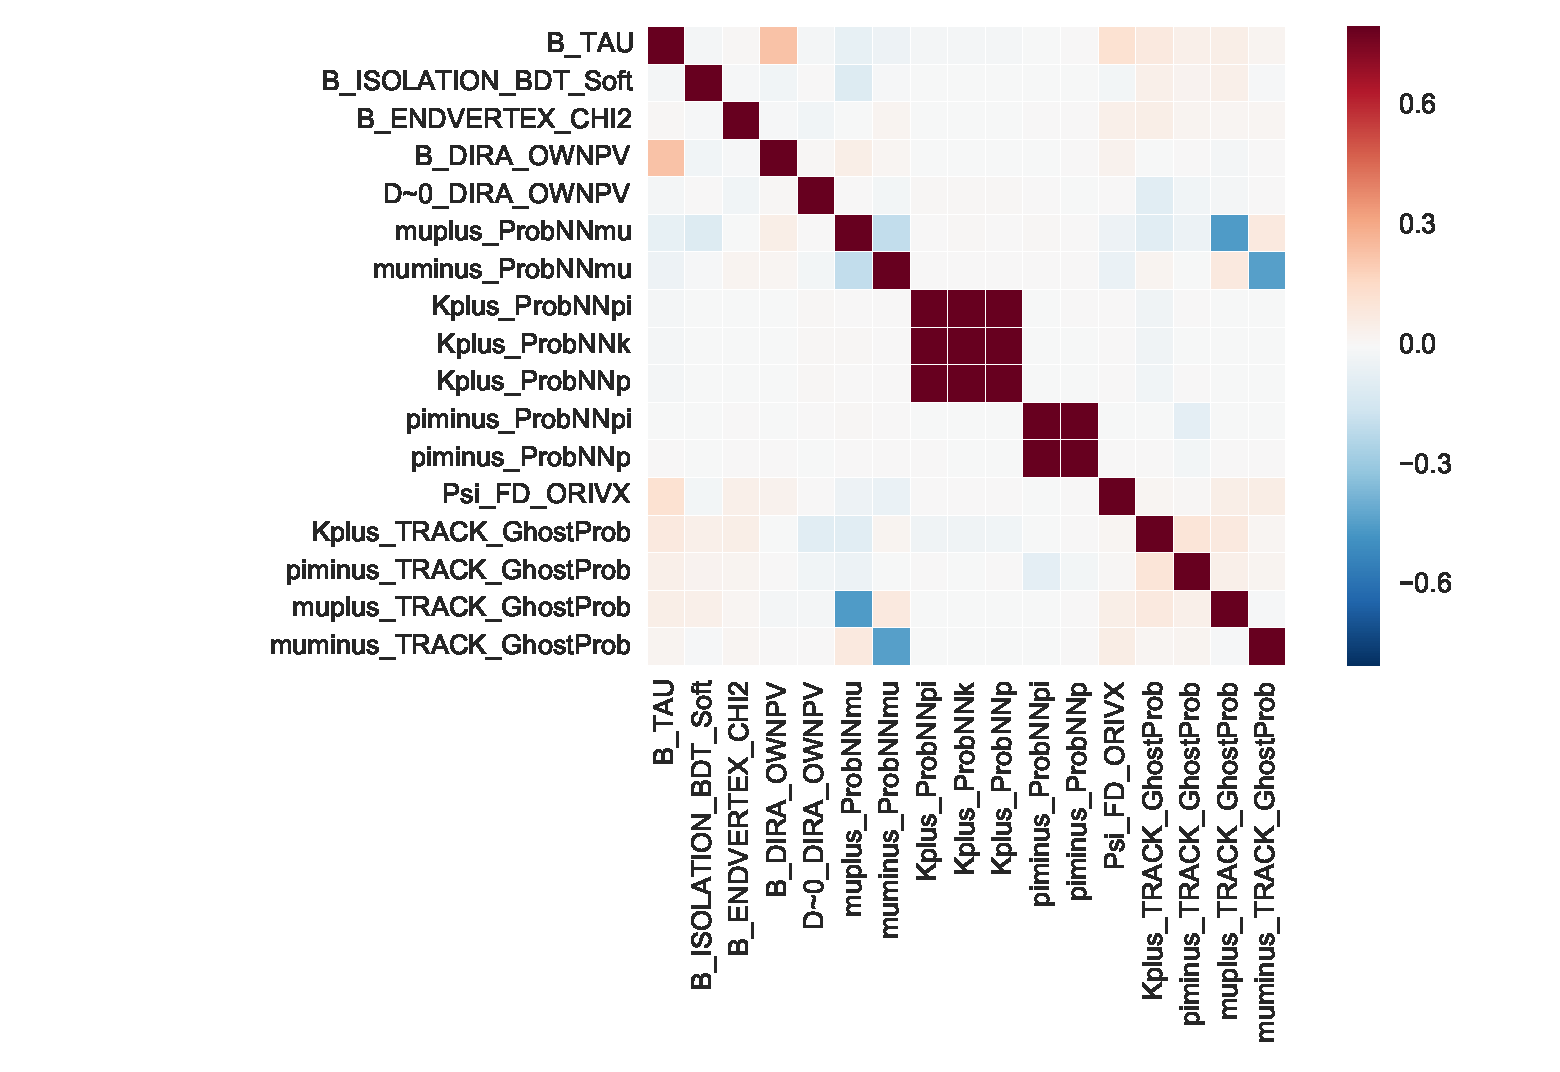
\includegraphics[page=1,width=\textwidth,trim=3cm 0cm 0cm 0cm,clip]{./figures/classifier.pdf}
  \end{minipage}
\end{frame}

\begin{frame}{Classifier: Feature importance}
  \centering
  \includegraphics[page=4,width=0.8\textwidth]{./figures/classifier.pdf}
\end{frame}

\begin{frame}{Classifier: ROC curve}
  \begin{minipage}{0.19\textwidth}
    \begin{itemize}
      \item 10-fold cross validation
    \end{itemize}
  \end{minipage}
  \begin{minipage}{0.8\textwidth}
    \centering
    \includegraphics[page=2,width=\textwidth]{./figures/classifier.pdf}
  \end{minipage}
\end{frame}

\begin{frame}{Classifier: Choice of $N_\text{estimators}$}
  \centering
  \includegraphics[page=3,width=0.8\textwidth]{./figures/classifier.pdf}
\end{frame}

\begin{frame}{Classifer: Test on \HepProcess{\PB\to\PKstar\Pmu\Pmu}}
  \begin{minipage}{0.35\textwidth}
    \begin{itemize}
      \item Monte Carlo is unreliable (PHSP) and signal is blinded \\
        \vspace{1em}
        $\Rightarrow$ Let's run the classifier on \HepProcess{\PB\to\PKstar\Pmu\Pmu}!
      \item Idea: Use this sample to investigate partial dependence
    \end{itemize}
  \end{minipage}
  \begin{minipage}{0.64\textwidth}
    \centering
    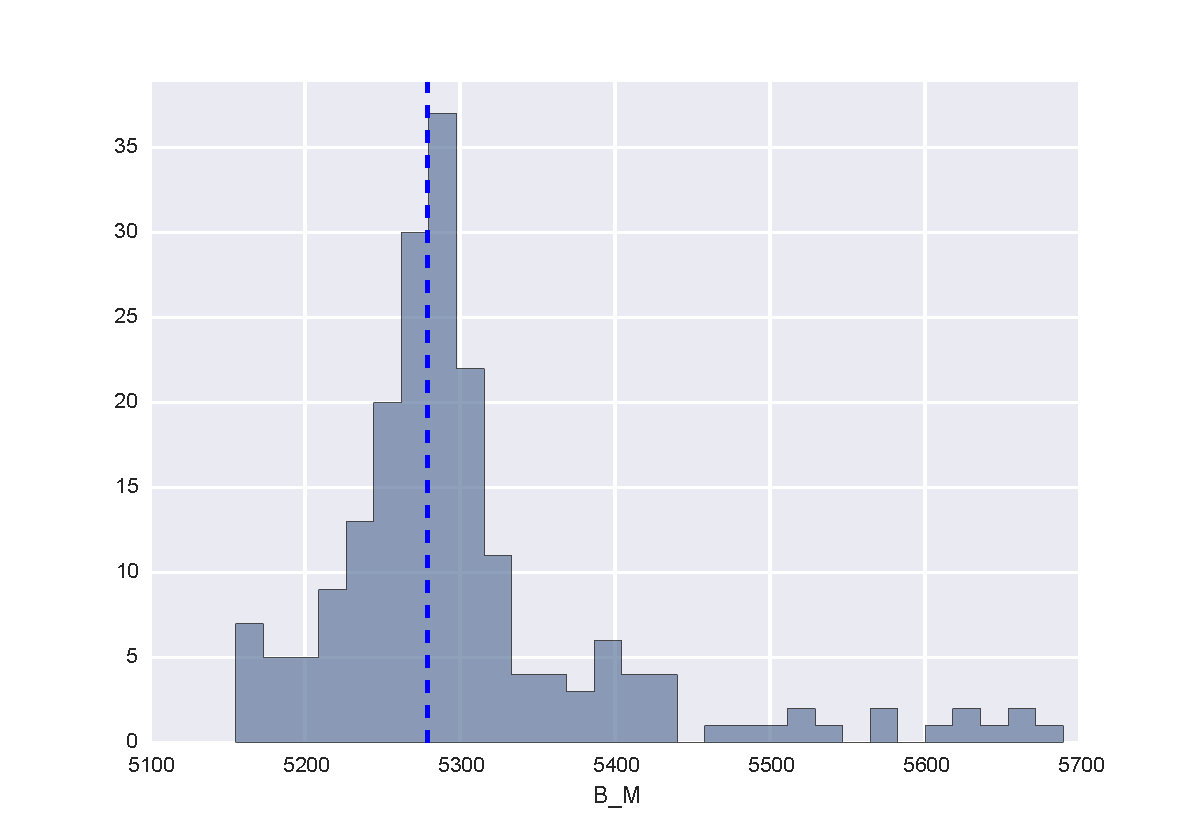
\includegraphics[page=1,width=\textwidth]{./figures/plots_kst.pdf}
  \end{minipage}
\end{frame}

\begin{frame}
  \begin{center}
    \Huge Thanks for listening!
  \end{center}
\end{frame}

\appendix

\begin{frame}{Backup (\PKstar decision function)}
  \centering
  \includegraphics[page=69,width=0.8\textwidth]{./figures/final.pdf}
\end{frame}

\begin{frame}{Backup (\PKstar masses)}
  \centering
  \makebox[\textwidth][c]{%
  \includegraphics[page=70,width=0.56\textwidth]{figures/plots_kst.pdf}%
  \includegraphics[page=71,width=0.56\textwidth]{figures/plots_kst.pdf}%
  }
\end{frame}

\begin{frame}{Backup}{\PDzero mass distribution after BDT}
  \centering
  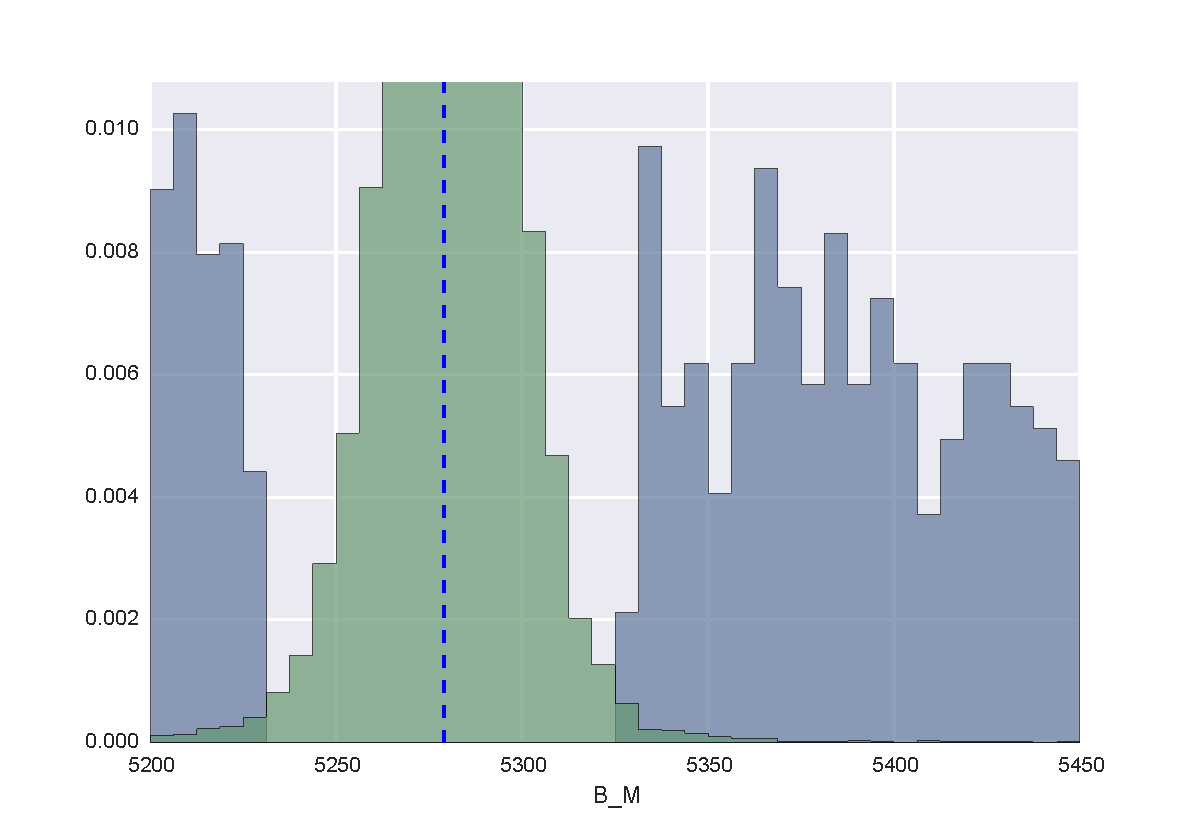
\includegraphics[page=1,width=0.8\textwidth]{./figures/final.pdf}
\end{frame}

\begin{frame}{Backup (\PDzero decision function)}
  \centering
  \includegraphics[page=69,width=0.8\textwidth]{./figures/final.pdf}
\end{frame}

\end{document}

